\chapter{Background}
\label{cha:background}
This chapter provides an overview of the text mining field along with previous work in the area and all necessary background information required to understand the major tasks involved in this project.

\section{Text Mining}
\label{sec:textmining}
The information available in the world is growing exponentially, and the majority of this information(widely estimated at roughly 80\%) is unstructured. This is where text mining comes in, also referred to as Knowledge Discovery from Text(KDT).
``Text mining is the process of extracting interesting information and knowledge from unstructured text"\cite{hotho-etal-ldv-2005} and its applications tend to work in two steps, first using an Information Retrieval(IR) application to narrow the search space, and then they extract significant parts of the retrieved texts\cite{Polajnar2006}. This general process usually involves structuring a source text by means of parsing and other linguistic analysis, then finding patterns in this structured data and then interpreting this output.

Text mining is fundamentally different from standard web searching in that web searches rely primarily on information that is already known. However, the goal of text mining is to discover interesting, previously unknown information\cite{Gupta_Lehal_2009}.
There is however one key issue introduced by text mining; natural language is used by humans for communication and recording information, while computers are incapable of interpreting natural language. Humans are naturally able to find linguistic patterns in text and understand the semantics of what is being said. Computers, on the other hand, face difficulties in interpreting variations in written text through spelling, colloquialism and also the general context of the text. Nonetheless, computers have what humans do not, that is, computers are much more capable of processing large datasets at very high speeds, particularly in comparison to the human being. Thus, the objective of text mining is to combine the best of these both by creating an application that can retrieve relevant documents and then apply linguistic patterns which may be rule-based, using human-defined rules, or taught by means of machine learning techniques. This project takes the rule-based approach and as such onlythese techniques will be discussed.

An example of the text mining process can be seen in Figure~\ref{fig:tm}.
\begin{figure}
\begin{center}
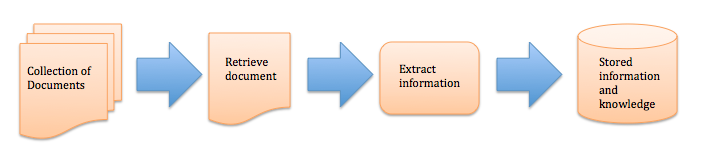
\includegraphics[width=15cm]{tm}
\end{center}
\caption{The text mining process\cite{Gupta_Lehal_2009}}
\label{fig:tm}
\end{figure}


\subsection[Information Retrieval]{Information Retrieval(IR)}
IR is the process of retrieving textual documents which may contain the answers to questions but do not answer these themselves\cite{hotho-etal-ldv-2005}. Information retrieval is fundamentally a web search working off user queries representing an information need. 


% MENTION MACHINE LEARNING V RULE/DICTIONARY BASED APPROACH
\subsection[Natural Language Processing]{Natural Language Processing(NLP)}
\subsubsection{Tokenisation}
\subsubsection{Part of Speech(POS)}
\subsubsection{Lemmatisation}
\subsubsection{Named Entity Recognition(NER)}

\subsection[Information Extraction]{Information Extraction(IE)}


\section[Sentiment Analysis]{Sentiment Analysis and Opinion Mining}

\section{Twitter Mining}
There has been several previous works on text mining Twitter posts, however, the bulk of these have focussed solely on biomedicine and the financial sector.


% MOVE TWITTER API HERE? FROM IMPLEMENTATION CHAPTER
